% =====================================================================
%  Slide-Examiner --- AAAI-27 anonymous submission
%  Build:  pdflatex main && bibtex main && pdflatex main && pdflatex main
%  Two-column AAAI camera-ready style. Anonymized via [submission].
%  Figures in ./figs/ (PNG data figs + PDF vector concept art w/ overpic).
% =====================================================================
\documentclass[letterpaper]{article}            % DO NOT CHANGE
\PassOptionsToPackage{table}{xcolor}            % columncolor in reward table
\usepackage[submission]{aaai2027}               % DO NOT CHANGE
\usepackage[hyphens]{url}                        % DO NOT CHANGE
\usepackage{graphicx}                            % DO NOT CHANGE
\urlstyle{rm}\def\UrlFont{\rm}
\usepackage{natbib}                              % DO NOT CHANGE / no options
\usepackage{caption}                             % DO NOT CHANGE / no options
\frenchspacing
\setcounter{secnumdepth}{2}   % AAAI-27 permits section numbers (Instructions L525); depth 2 so subsection \ref{sec:g7,elicit,coverage} resolve

\usepackage{amsmath}
\usepackage{amssymb}
\usepackage{booktabs}
\usepackage{array}
\usepackage{multirow}
\usepackage[percent]{overpic}    % text overlays on vector concept art
\definecolor{figink}{HTML}{2B3440}
\definecolor{figslate}{HTML}{5A6675}
\definecolor{figblue}{HTML}{3F6FB5}
\definecolor{figorange}{HTML}{E07F2C}
\definecolor{figred}{HTML}{D24A43}
\definecolor{figgrey}{HTML}{9AA4B0}
\definecolor{figteal}{HTML}{2A9D8F}
\definecolor{figpurple}{HTML}{7A5DBB}

\newcommand{\g}[1]{\textsf{#1}}        % defect-class names
\newcommand{\best}[1]{\textbf{#1}}
\newcommand{\ci}[1]{\,{\scriptsize[#1]}}   % compact 95% Wilson interval

\pdfinfo{/TemplateVersion (2027.1)}

\title{Diagnose Before You Inspect:\\
Failure Attribution Prescribes a Deterministic\\
Symbolic--Neural Critic for Slides}
\author{Anonymous Authors}
\affiliations{}

\begin{document}
\maketitle

\begin{abstract}
\noindent
Vision--language models (VLMs) routinely pass slides with visible defects, but a failed inspection does not
identify why the model failed. We test whether separating failure mechanisms can determine the appropriate
inspection method. Using a structured-geometry oracle that is lossless with respect to the declared IR, we distinguish defects
that fall below the models' effective perceptual threshold, defects that are visible but suppressed by a whole-rubric prompt, and
\emph{reference-assisted} defects that become resolvable only when a clean twin is available. The resulting
critic assigns declared geometry and terminology to symbolic linters, format-suppressed defects to atomic VLM
queries with required evidence, reference-assisted defects to paired comparison, and page semantics to a
finetuned examiner. On three vendors, atomic elicitation outperforms a compute-matched self-consistency baseline
with a single call. The deterministic composition reaches 0.957 macro balanced accuracy on held-out validation.
A later frozen check on a disjoint set scores lower when unresolved reference requests count as misses. Clean
controls for the reference-assisted class, pixel-recovered structure, and real \textsc{SlideAudit} layouts
identify the conditions under which this assignment transfers.
\end{abstract}

\begin{figure}[!t]
\centering
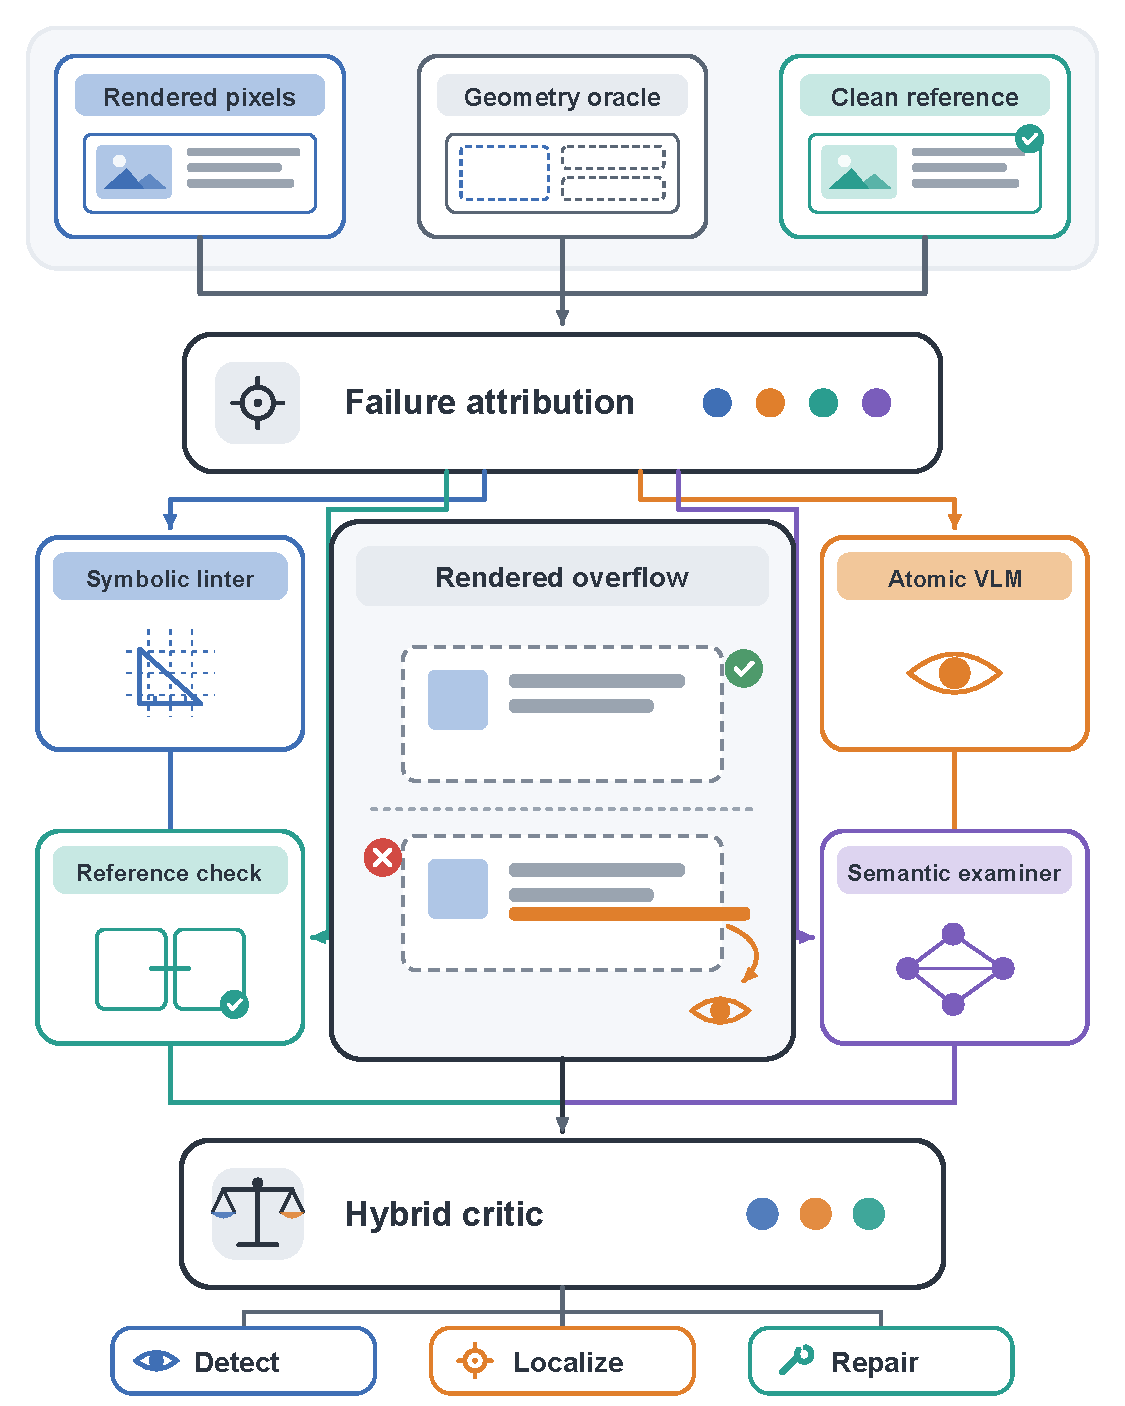
\includegraphics[width=0.94\columnwidth]{figs/fig_teaser.pdf}
\caption{\textbf{Diagnose before inspection.}
A geometry oracle attributes each failure, then routes it to symbolic linting, atomic VLM elicitation,
reference comparison, or semantic examination for deterministic fusion by the hybrid critic.}
\label{fig:teaser}
\end{figure}

% =====================================================================
\section{Introduction}
% =====================================================================

Slide- and document-generation agents need critics that can locate layout and content defects before an output
is returned or revised. A common choice is a general-purpose vision--language model (VLM) prompted to grade the
rendered slide against a rubric. Yet the resulting judgment does not reveal why a defect was missed. For
example, a strong VLM may answer ``no defect'' when a title visibly spills out of its box. The same answer is
consistent with two different failures: the model may not resolve the overflow, or the prompt may fail to elicit
a signal the model can use. These explanations imply different remedies, ranging from better visual input to a
different query or a symbolic tool.

This distinction becomes more important when defects vary in scale and in the evidence required to identify
them. Some defects are \emph{sub-perceptual} under the tested protocol, such as a three-pixel alignment offset
or a one-point font mismatch below the models' effective acuity. Changing the prompt, scale, or resolution does
not recover them. Other defects are \emph{format-suppressed}: the model detects them when asked one targeted
question with required evidence, but misses them when one pointwise call must score the full rubric. A third
set is \emph{reference-assisted}. These defects become resolvable when the model can compare the slide with a
clean twin, but not from the single slide alone. Treating all three outcomes as generic failures of ``visual
understanding'' obscures which intervention is appropriate.

We measure this distinction with an attribution protocol based on a structured-geometry oracle that is lossless with respect to the declared IR.
Each slide has an intermediate representation (IR) containing element bounding boxes, text, and style. We
present matched defective and clean slides as an image, the structured oracle, a VLM-generated caption, or the
image together with the oracle. We cross these inputs with detection, localization, and repair tasks. Unlike a
model-generated caption, the oracle exposes the declared structure without first passing it through another
visual model. Success with the oracle after failure on the image therefore operationally identifies a
perception bottleneck at the tested interface. Failure with both inputs indicates that changing the neural input
alone does not solve the class.

The attribution results determine a fixed division of labor (Fig.~\ref{fig:teaser}). Symbolic linters inspect
declared geometry and terminology. A language model handles text and structural semantics. VLMs inspect
perceivable defects under the elicitation format supported by the diagnosis, using either an atomic query or a
clean reference. We also construct \g{G7}, a render-containment overflow whose declared box is legal although
its rendered content crosses the boundary. This class tests the part of the design that a structure-only linter
cannot observe. The complete symbolic--neural critic assumes an IR-owning generation agent. When only
third-party pixels are available, the linter lacks its required input and the available critic reduces to the
re-elicited VLM (Sec.~\ref{sec:external}).

The paper makes four connected contributions. First, the structured-oracle protocol separates sub-perceptual,
format-suppressed, and reference-assisted failures, and we repeat the attribution on real CC-licensed layouts
(Secs.~\ref{sec:diag} and~\ref{sec:external}). Second, defect-specific elicitation recovers signals suppressed
by a whole-rubric prompt, whereas \g{G1} text overflow and \g{S6} image/text contradiction still require a clean
reference (Sec.~\ref{sec:hybrid}). Third, a compute-matched control shows that this recovery is not explained by
additional test-time compute: for \g{G7}, one atomic call exceeds ten-draw self-consistency by 0.20--0.31 across
three vendors. Finally, the resulting deterministic composition, which uses no learned assignment model,
reaches 0.957 macro balanced accuracy on held-out validation. A later frozen image-arm check reaches 0.826 on a
disjoint set when unresolved reference requests count as misses. Clean-control errors, failed structure
recovery, and transfer to real layouts define the scope of these results.

% =====================================================================
\section{Related work}
% =====================================================================

\paragraph{The VLM perception bottleneck.}
Prior work separates several sources of visual failure. Chart understanding can be limited either by the
vision encoder or by extraction from its representation~\citep{chartbottleneck}. Direct readouts likewise show
that visual information available in an encoder may not be used effectively by the full VLM~\citep{hiddeninplainsight}.
\textsc{MMVP} constructs image pairs that expose systematic shortcomings associated with CLIP-based visual
representations~\citep{mmvp}. We study quality inspection of generated artifacts, where declared geometry
provides a structured observation of the visual content and the attribution result can be used to choose the
critic's inspection method.

\paragraph{Perception/reasoning attribution.}
Concurrent work uses natural-language descriptions to separate perception from reasoning in abstract
visual-reasoning benchmarks~\citep{reasoningbench}. Our setting instead provides a structured representation of
boxes, text, and style, together with exact labels from controlled injection. The representation avoids using a
caption as the oracle and lets the attribution select a downstream inspection method. The \textsc{LED}
benchmark also injects empirically grounded structural errors, but it evaluates errors in document-layout-analysis
predictions and studies limitations of overlap-based metrics~\citep{led}. We inject errors into rendered slide
artifacts and use the resulting diagnosis to compose a critic.

\paragraph{Relative vs.\ absolute judgement.}
VLM judges can preserve rankings while producing uncertain absolute scores~\citep{rankscore}.
Pairwise assessment has also improved zero-shot NLG evaluation for some LLMs, although it exhibits positional
bias~\citep{comparative}. Protocol choice can introduce other biases as well: pairwise judgments may be more
sensitive than absolute scores to distractor features~\citep{pairpoint}. Our experiments use relative and atomic
queries as diagnostic interventions rather than assuming that either is generally superior. The useful result
is their class boundary: they recover \g{G1} text overflow and \g{S6} image/text contradiction, but not fine
\g{G3} alignment or \g{S3} terminology drift.

\paragraph{Slide generation, evaluation, and reward.}
Recent slide systems combine generation with evaluation or revision. AutoPresent studies programmatic slide
generation and iterative self-refinement~\citep{autopresent}. AeSlides optimizes layout with verifiable aesthetic
rewards~\citep{aeslides}, while EvoPresent uses an aesthetic model for scoring, adjustment, and comparative
feedback~\citep{evopresent}. \textsc{VLM-SlideEval} tests element extraction, perturbation sensitivity, and
narrative ordering, and argues for calibrated critics in iterative pipelines~\citep{vlmslideeval}.
\textsc{SlideAudit} contributes an expert-derived defect taxonomy and annotated slides for evaluating design
critique~\citep{slideaudit}. We use its taxonomy and real slides for transfer evaluation, then audit five
published scorers and one closed VLM judge on the constructed render class (Sec.~\ref{sec:g7}).

% =====================================================================
\section{Problem setup and defect taxonomy}\label{sec:setup}
% =====================================================================

\paragraph{Task and representation.}
The critic inspects a single rendered slide, optionally with its declared structure, and must \emph{flag and
localize} defects of a fixed set of types; a detection counts only when it fires on a defective slide and stays
silent on its matched clean twin. Every slide is an intermediate representation (IR) of typed elements with
bounding boxes, text, and style; we inject defects programmatically into the IR and render, yielding exact
labels and matched (defective, clean) pairs. The taxonomy (Table~\ref{tab:taxonomy}) has a \emph{geometry}
group \g{G1}--\g{G6}, a \emph{semantic} group \g{S1}--\g{S6}, and one constructed render class \g{G7}; it is
aligned to the expert-derived \textsc{SlideAudit} taxonomy~\citep{slideaudit} via a bidirectional map (crosswalk in
the supplement), and results are reported in its canonical classes. We add \g{G7} to test the linter's blind spot: the declared box is legal (inside the safe margin, no
overlap) but the rendered content overflows its container, so the defect exists \emph{only} in pixels. On real
agent-generated decks \g{G7} is common, affecting most slides of a Zenodo10K slice and over half of an
AutoPresent slice.\footnote{93-deck Zenodo10K slice: 81/93 decks affected (857/3167 legal boxes); 14-deck
AutoPresent slice: 8/14 decks (20/50 legal boxes).}

\begin{table}[tb]
\centering
\small
\caption{Defect taxonomy. The geometry group is detected symbolically; the semantic group is the examiner's
domain; \g{G7} is constructed to be linter-blind. ``Channel'' is the engine the diagnosis assigns
(Sec.~\ref{sec:diag}--\ref{sec:hybrid}).}
\label{tab:taxonomy}
\setlength{\tabcolsep}{4pt}
\resizebox{\columnwidth}{!}{%
\begin{tabular}{@{}llll@{}}
\toprule
Group & Class & Description & Channel \\
\midrule
\multirow{6}{*}{Geometry} & \g{G1} text overflow & text exceeds its box & VLM+linter \\
 & \g{G2} element overlap & boxes intersect & linter \\
 & \g{G3} alignment offset & small mis-alignment & linter \\
 & \g{G4} font-size inconsistency & off-grid font size & linter \\
 & \g{G5} brand-color violation & off-palette color (CIELAB color difference $\Delta E$) & linter \\
 & \g{G6} margin violation & element past safe margin & linter \\
\midrule
\multirow{6}{*}{Semantic} & \g{S1} title/body mismatch & body contradicts title & VLM \\
 & \g{S2} narrative-order break & deck sections out of order & LLM \\
 & \g{S3} terminology inconsistency & term drift across deck & term linter \\
 & \g{S4} density violation & slide over/under-packed & LLM \\
 & \g{S5} missing logic section & dropped argument step & LLM \\
 & \g{S6} image/text contradiction & figure contradicts caption & VLM \\
\midrule
Render & \g{G7} containment overflow & legal box, rendered overflow & VLM (atomic) \\
\bottomrule
\end{tabular}}

\end{table}

\paragraph{Attribution modalities and metric.}
To attribute a failure, we define four input conditions. Condition A contains only the rendered image.
Condition B contains the structured oracle, which preserves element boxes, text, and style from the source
IR without loss. Condition B$'$ contains a VLM-written caption and serves as a lossy control. Condition C combines the image
and oracle. Under each condition, we ask the model to detect, localize, and repair the defect. The attribution reads off the A-vs-B contrast: if
the model fails on the image alone (A) but succeeds given the oracle (B), we call the class
\emph{perception-bottlenecked} operationally: the task becomes solvable when the same information is made
explicit in structure that is lossless with respect to the declared IR. This is a diagnosis of which engine can solve the class, not a claim about the
model's internal representations. If it fails under both, the class is unsolved even at the structured
interface, and we assign it to a symbolic method.\footnote{The oracle's ground-truth labels are stripped from the model's view by a
regression-tested de-leaking pass, so B tests perception of structure, not label leakage. B$'$ is a control,
not a second oracle: a caption re-injects the perceptual error it is meant to factor out, so B's advantage is
by construction.} We report \emph{balanced accuracy on the paired clean controls}: a detection
counts only if it fires on the defective slide and stays silent on its matched clean twin, so a model cannot
score by flagging everything.

\paragraph{Two linters.}
A geometry linter detects \g{G1}--\g{G6} from coordinates and rules (brand color via CIELAB $\Delta E_{2000}$, not RGB
distance), at zero false positives on clean slides. A terminology linter handles \g{S3} from an occurrence
table plus near-duplicate clustering, image-free. Both are the ``detectors of record'' prescribed by the diagnosis.

% =====================================================================
\section{Diagnosis: two kinds of blindness}\label{sec:diag}
% =====================================================================

\paragraph{Pointwise image-only inspection misses fine geometry.}
Under the conventional setup, one slide receives one rubric score with no reference slide for comparison. We
call this \emph{pointwise image-only} inspection. In this setting, \g{G2}--\g{G6} sit at chance for 4B and 8B models, and a 30B breaks only
\g{G1} overflow. The floor remains under the tested changes: swapping the vision encoder across \emph{five}
families (SigLIP2, an LLM-based encoder, InternViT, a native-resolution NaViT, MoonViT) leaves every model at
the random line (differing only in abstain-vs-over-flag bias), and raising resolution 1536$\to$2048 changes
nothing. The lever is elicitation and magnitude, not encoder or pixel budget, so the floor is a property of
the \emph{pointwise} protocol, not a hard capability limit. For declared geometry, the symbolic linter reads coordinates directly and reaches balanced accuracy 0.75--1.0
with zero false positives where the IR is available.

\paragraph{Some apparent perceptual failures depend on elicitation.}
The same setting hides a second, opposite phenomenon. For \g{G1} overflow and \g{S6} image/text contradiction,
pointwise balanced accuracy is 0.50, indistinguishable from the sub-threshold tail, yet a
two-alternative forced choice between the defective and clean slide jumps to 1.00: the defect is perceivable,
but the single-slide pointwise call does not surface it. We therefore treat \g{G1}/\g{S6} as
\emph{reference-assisted}: recovery needs the clean twin, not just a renamed single-image question. \g{G3}
alignment behaves differently, but only \emph{above a magnitude threshold}: sweeping the injected offset as an
internal contrast (one element shifted from its aligned sibling column), the forced choice saturates to $1.00$
by $16$\,px ($0.83\%$ of slide width) while the sub-threshold tail ($\le8$\,px) stays at chance even side by
side. So fine alignment is not a class-level capability floor: above threshold it is format-suppressed and
recoverable, with a sub-perceptual residue only in the small-offset tail. The connecting thread is a
\emph{magnitude-gated} recoverable-versus-sub-perceptual boundary rather than a clean geometric/semantic split,
and \g{S3} terminology (below) remains the one defect no elicitation rescues.

On the rebuilt corpus we also now have a human spot-check on the actual pairs cited here, not just the earlier
diagnosis runs. Replacing only the stale legacy \g{G3}/\g{G5} samples and keeping the other 55 pairs fixed,
the v2 pass verifies every sampled defect as visible and every clean twin as clean (73/73, Wilson lower bound
0.95 for both), with source-structure faithfulness 55/55 on the auditable classes. The delta is exactly where
the re-operationalisation says it should be: \g{G3} shifts from 0/7 on the old external-reference sample to
8/8 on the corrected within-list misalignment sample, and \g{G5} from 0/7 to 10/10 on the corrected
within-list chromatic clash sample; the non-replaced 55 pairs are unchanged.

\paragraph{Terminology remains unresolved.}
Not every consistency defect is format-suppressed. \g{S3} terminology inconsistency is \emph{not} rescued by
forced choice (0.625, heavy position bias): reading the same term across deck pages and spotting a subtle
variant is below threshold even side by side. The structured-oracle channel, which feeds the model
the full deck text with both variants present, also fails (0.56): with both variants already explicit in the
input, this failure cannot be OCR, and instead reflects cross-page term-matching that does not survive the
yes/no framing. The image channel is consistent with fine-grained glyph discrimination and the oracle channel
fails even with the text in hand, so neither neural method is reliable. \g{S3} is therefore assigned to a symbolic terminology linter,
which reaches balanced accuracy 1.000 against the VLM's 0.69, a negative result that changes the prescribed method.

\paragraph{The \g{G6} page-offset boundary depends on magnitude.}
Re-posing a defect as a within-slide contrast does not rescue every class. It fails outright on \g{G6}. We
redefine \g{G6} margin as a \emph{page offset}: the whole content block is shifted toward one edge (every
element together, so internal alignment is preserved and the defect cannot be misalignment), leaving one
margin crowded against (or running off) the edge and the opposite side empty.\footnote{The original \g{S6}
render omitted the figure element, so the cross-modal contradiction was literally unseeable (recall $0$); on
the valid-figure corpus the \g{S6} 2-AFC reproduces at $0.75$--$1.00$ across all six VLMs, confirming it is a
render artifact, not blindness.} Across all six VLMs and both pointwise framings the page offset stays at
chance (roster-mean C3 $0.50$), and the pairwise test that separates \emph{data artifacts} (\g{S6}, which
recovers to perfect once the figure is rendered) from genuine blindness leaves \g{G6} on the floor for
\emph{every} model. A stress-test addendum identifies the boundary: when the same rigid offset moves
content 48 px beyond the page edge, both C0 and C3 detect the defect at 0.958 balanced accuracy (11/12 positives,
12/12 clean controls), although C0 never names \g{G6} while C3 does. Thus the blind spot is genuine over the
tested moderate, unclipped range but not magnitude-invariant; overt clipping restores visibility. Declared
geometry is still assigned to the linter because it detects both regimes without relying on this visual threshold.

\paragraph{Template snapping can remove injected defects.}
Enterprise ``snap-to-master'' templates re-fit element boxes to a grid before rendering, and we find a
template silently \emph{absorbs} 45\% of injected geometry defects: overlap, alignment, and margin violations
become pixel-identical to their clean twins after snapping, while overflow (content-determined) survives, a
trap for any dataset that derives labels from the IR but evaluates on the rendered image, quantified and tied
to a reward-model failure in Sec.~\ref{sec:g7}.

% =====================================================================
\section{From diagnosis to a deterministic symbolic--neural critic}\label{sec:hybrid}
% =====================================================================

The diagnosis says a single model is the wrong unit. We prescribe a fixed correspondence from diagnosed failure
type to inspection method, validate the elicitation recovery across models, and stress the composition with the
constructed render class \g{G7}. This assignment is deterministic, not learned from class outcomes.

\subsection{Elicitation separates format suppression from unresolved capability limits}\label{sec:elicit}

\paragraph{Four ways to ask.}
Holding the model and image fixed, we compare four prompting conditions. C0 is one call that scores every
defect type against a rubric. C1 asks for a free-form description before classification. C2 uses a
synthetic-twin pair in which the clean reference is re-rendered to a grid. C3 issues one yes/no query per defect
type and requires localization of the offending element. The primary comparison is C3 against C0. The model,
image, and taxonomy remain fixed; only the whole-rubric versus atomic evidence-bearing format changes. A gain
under C3 therefore identifies sensitivity to the elicitation format under this controlled comparison.

\paragraph{C3 recovers \g{G7} within the capable subset.}
We scope the claim to models that can see \g{G7} at all: a model counts as ``capable'' only if, under C3, it
both detects the overflow (balanced accuracy $\ge0.70$ and precision $\ge0.70$ on paired clean controls) and
points at the overflowing element; selected on the same test items, this subset is descriptive rather than
confirmatory. This excludes InternVL-8B and Ovis-9B, which stay near chance, a
capability boundary rather than a format effect. On the four capable models (three scales, three vendors), C3
recovers what C0 suppresses: balanced accuracy $0.50$--$0.79\!\to\!0.93$--$1.00$, precision $0.88$--$1.00$.
The effect appears across models. Pairing each slide across the four models, C3 fixes 233 \g{G7} items that C0
missed against 2 reversals (McNemar $\chi^2_1{=}227$, $p<10^{-50}$).\footnote{Per-model $p\le1.5\!\times\!10^{-11}$,
all surviving Holm correction over the final paper-wide 85-test family; the two reversals are on Gemma4-31B
(C3 recall $88/90$). Full table in the supplement.} C0's one-call rubric does not include \g{G7}, which is a render class outside the original taxonomy. C3 asks
about that class directly. The next controls separate the effect of naming the class from the effect of using an
atomic query.

\paragraph{Naming and query format have different effects.}
Is it naming the class that helps, or changing how we ask? Two controls separate this. \emph{C0+} is C0 with
\g{G7} added to the rubric's defect list. It retains the one-call format but gives the model a name for the
class. \emph{C0\_named} instead asks about \g{G7} alone, on its own yes/no call. Table~\ref{tab:format} shows the split. Adding the name to the one-call rubric (C0+) recovers recall (234
defectives newly flagged, $p{=}7\!\times\!10^{-71}$), but it reduces specificity: clean slides are over-flagged
on 55\% of pairs, compared with 2.4\% for C3, so balanced accuracy remains lower. Asking about \g{G7} on its own call (C0\_named) recovers
both, and supplying a clean reference slide adds nothing on top. So for \g{G7} the suppressor is the
\emph{one-call format}: under a targeted atomic query, the same model on the same image recovers the detection
the whole-taxonomy rubric buries. The boundary is \g{G1}/\g{S6}: naming alone does \emph{not}
help. Those classes need the clean reference slide (pairwise choice $\to0.97$--$1.00$), a
\emph{reference-assisted} effect rather than single-slide format suppression. A clean-vs-clean control rules out a
forced-pick artifact (capable models answer ``tie'' on $92$--$100\%$ of clean pairs).

\paragraph{The recovery persists under compute matching.}
The remaining alternative is that C3 wins only because it spends more test-time compute than the one-call rubric.
We test that directly on three API-served models spanning distinct vendors, holding the image and rendered corpus
fixed and matching C3's budget with repeated C0 draws. The compute-matched control is \emph{self-consistency}: majority
vote over $K{=}10$ independent C0 samples. On \g{G7}, C3 still beats that compute-matched control on all three
vendors ($0.92/0.88/0.83$ vs. $0.61/0.59/0.63$; $\Delta{=}+0.31/+0.29/+0.20$), and all three contrasts survive
Holm correction within the full 24-test family (reported in the supplement). The budget points the same way:
C3 is the cheapest condition in completion tokens ($34.7/37.5/40.5$ output tok per slide, one call) while the
matched self-consistency baseline spends 8--10 calls per slide and still loses. A larger sampling budget therefore does not account for the recovery in this experiment. Changing the
whole-taxonomy pointwise format recovers detection without increasing test-time compute. We report the union aggregation of the same draws, the
definition-matched one-call control, and the \g{G1} negative control in the supplement.

\begin{table}[tb]
\centering\small
\setlength{\tabcolsep}{4pt}
\caption{Naming vs.\ format on \g{G7}. Adding the class name to the one-call rubric (C0+) recovers recall
but wrecks specificity (55\% clean over-flag); asking about \g{G7} on its own call (C0\_named, C3) recovers
both. C0\_named matches C3, so a clean reference adds nothing for \g{G7}.}
\label{tab:format}
\setlength{\tabcolsep}{3pt}
\begin{tabular}{@{}p{0.46\columnwidth}cc@{}}
\toprule
elicitation (\g{G7}) & clean over-flag & bal-acc \\
\midrule
C0 (whole-tax., unnamed)      & 2.4\% & 0.50 \\
C0+ (whole-tax., \g{G7} named) & 55\% & 0.58--0.82 \\
C0\_named (atomic, no ref.)   & 2.4\% & \best{0.93--1.00} \\
C3 (atomic, +forced loc.)     & 2.4\% & \best{0.93--1.00} \\
\bottomrule
\end{tabular}
\end{table}

\paragraph{Elicitation depends on model capability and defect class.}
The best elicitation depends jointly on model capability and defect class. No single prompt covers all cases, so
inspection must be assigned per diagnosed failure: the C2 synthetic-twin pairwise rescues declared \g{G1} on capable
models (snapping absorbs the overflow and the contrast exposes it), while C1 free-form rescues weak models
but collapses on strong ones (precision $\approx0.50$). The format effect is not a synthetic artifact: on
human-annotated \textsc{SlideAudit} (no structure) C3 still beats C0 for every class (e.g.\ brand color,
alignment). Absolute geometry on bare real pixels stays modest outside blatant overlap. Real fine geometry
needs the linter, hence the structure bare images lack, so on image-only real data the hybrid degrades to
VLM-only, a ceiling set by missing structure, not method.

\subsection{The minimal hybrid critic covers the most}\label{sec:coverage}

\paragraph{The assigned methods provide complementary coverage.}
On a separate novel-template held-out validation set ($150$ positives and $150$ clean controls per
class), the corrected deterministic composition reaches macro balanced accuracy .957 and
covers 8/9 classes; the sole miss is \g{S6} (.677 balanced accuracy, .607
precision), whose perfect recall is offset by clean false positives (full table
and fidelity audit in the Technical Supplement).
On a later disjoint seed-controlled set generated after the method assignment was frozen ($30$ positives and
$30$ clean controls per class), the completed frozen image arm scores macro balanced accuracy .826 and named
localization .778, with unresolved clean-reference requests counted as misses. These are distinct stages and
datasets: the former is held-out validation whose results had already been inspected, while the latter is a
separate frozen check rather than a rerun on that corpus.
We score each critic by \emph{named attribution}: a detection is correct only if it names the right defect
type on the defective slide and stays silent on the matched clean slide. We call a class ``covered'' when this
balanced accuracy exceeds 0.75 (with the 95\% Wilson lower bound above 0.65, so the cell is not just lucky).
Coverage tracks the diagnosis: declared geometry is covered by the linter, the format-suppressed classes by a
C3-elicited VLM. The mean balanced accuracy summarizes this complementary coverage. The minimal hybrid of a linter and one
C3-elicited VLM reaches 0.86, compared with 0.59 for the conventional pointwise VLM-C0 and 0.66 for the linter
alone (Table~\ref{tab:coverage}). Under the same strict covered criterion, the
minimal hybrid clears 6 of the 9 image-level classes; \g{G6} at 0.75\ci{.67,.80} misses by the paper's own
``exceeds'' rule, and \g{S1} under linter+C3 misses because its lower bound stays below 0.65. The nine classes
are the image-level ones; \g{G4}/\g{S3} are linter-owned and \g{S2}/\g{S5} are deck-scope
(Sec.~\ref{sec:examiner}). Note that this assignment needs no per-class tuning: the rule follows from the
diagnosis, not from optimizing over class outcomes, so the coverage table is what the diagnosis predicts rather
than a tuned architecture.

\begin{table}[tb]
\centering\scriptsize
\setlength{\tabcolsep}{2.5pt}
\caption{Per-class named-attribution balanced accuracy [95\% Wilson]; $n$ = paired positives (G1 40, G2 40, G3
70, G5 40, G6 80, G7 40, S1 18, S4 36, S6 12; precision per cell in the Technical Supplement). The minimal
linter+VLM-C3 hybrid has the highest mean balanced accuracy. ``covered'' means bal-acc $>0.75$ and Wilson
lower bound $>0.65$; under that rule, linter+VLM-C3 and the prescribed composition each clear 6/9 classes.
The prescribed column reports the corrected \g{S1} method; the frozen text-only \g{S1} baseline (0.25, precision 0.09)
is reported in the prose below. Small \g{S1}/\g{S6} cells are method-selection diagnostics, not confirmatory (those
claims rest on the elicitation decomposition and 2-AFC).}
\label{tab:coverage}
\setlength{\tabcolsep}{2.5pt}
\resizebox{\columnwidth}{!}{%
\begin{tabular}{@{}lccccc@{}}
\toprule
Class & linter & VLM-C0 & VLM-C3 & linter+C3 & prescribed \\
\midrule
\g{G1} overflow      & 1.00\ci{.91,1} & 0.50\ci{.46,.54} & 0.50\ci{.46,.54} & \best{1.00\ci{.91,1}} & \best{1.00\ci{.91,1}} \\
\g{G2} overlap       & 0.80\ci{.68,.87} & 0.71\ci{.60,.79} & \best{0.86\ci{.74,.92}} & 0.80\ci{.68,.87} & 0.80\ci{.68,.87} \\
\g{G3} alignment     & 0.93\ci{.85,.96} & 0.62\ci{.55,.68} & 0.71\ci{.63,.77} & \best{0.93\ci{.85,.96}} & \best{0.93\ci{.85,.96}} \\
\g{G5} color         & 1.00\ci{.91,1} & 0.50\ci{.46,.54} & 0.68\ci{.57,.75} & \best{1.00\ci{.91,1}} & \best{1.00\ci{.91,1}} \\
\g{G6} margin        & 0.75\ci{.67,.80} & 0.51\ci{.40,.61} & 0.51\ci{.47,.55} & \best{0.75\ci{.67,.80}} & \best{0.75\ci{.67,.80}} \\
\g{G7} render-overflow & 0.00\ci{0,.54} & 0.50\ci{.46,.54} & \best{1.00\ci{.91,1}} & \best{1.00\ci{.91,1}} & \best{1.00\ci{.91,1}} \\
\g{S1} title/body    & 0.50\ci{.41,.59} & \best{0.94\ci{.75,.98}} & 0.83\ci{.63,.92} & 0.83\ci{.63,.92} & \best{0.94\ci{.75,.98}} \\
\g{S4} density       & 0.50\ci{.45,.55} & 0.51\ci{.44,.59} & \best{0.93\ci{.81,.97}} & \best{0.93\ci{.81,.97}} & 0.72\ci{.60,.80} \\
\g{S6} image/text    & 0.50\ci{.38,.62} & 0.50\ci{.38,.62} & 0.50\ci{.38,.62} & 0.50\ci{.38,.62} & 0.50\ci{.38,.62} \\
\midrule
mean / covered & 0.66 \,/\, 4/9 & 0.59 \,/\, 1/9 & 0.72 \,/\, 3/9 & \best{0.86 \,/\, 6/9} & 0.85 \,/\, 6/9 \\
\bottomrule
\end{tabular}
}
\end{table}

\paragraph{The \g{S1} diagnosis changes its assignment.}
We initially assigned \g{S1} title/body mismatch to the text LLM, but the text-only probe over-flags (0.25,
precision 0.09) while the image-bearing VLM names it reliably (0.94, precision 0.90): title/body mismatch
needs the \emph{rendered layout}, not just the text. We therefore report both numbers: the frozen text-only
baseline and the corrected VLM method. Under the corrected assignment, \g{S1}
uses the VLM under its open pointwise prompt (C0, 0.94) rather than C3 (0.83), since recall is already
saturated and C3 only adds false positives. This case shows how the diagnosis changes method selection. The one
image-level class the hybrid does not cover is \g{S6} image/text contradiction, at 0.50 single-image for every
engine; the pairwise test shows the model \emph{does} perceive it (recall 1.0, specificity $\sim$0,
over-asserting rather than missing), so this is a reference-assisted effect, not a blind spot, in contrast to
the moderate, unclipped \g{G6} page-offset regime.

\subsection{\g{G7}: the linter-blind class that specialised rewards also miss}\label{sec:g7}

\paragraph{Construction and scorer response.}
\g{G7} makes the linter's blind spot falsifiable: a declared box that is legal (in-margin, non-overlapping) but
whose rendered content overflows its container. The IR carries only legal short text; the overflow lives in the
renderer, so the linter and any structure-only model are blind by construction. A self-check confirms zero
findings on 90/90 \g{G7} defectives. We then audit five published scorers plus one frontier VLM judge on the
same paired slides. The same-backbone comparison provides the most direct separation: CLIP-IQA detects \g{G7}, whereas the LAION
aesthetic head on the same CLIP-L/14 backbone is at chance. Skywork, PickScore, and Qwen3.7-Max also detect the
class, whereas DocReward does not (full per-scorer table in the Technical Supplement). So on the
scorers tested, \g{G7} tracks a rendered-quality read-out rather than the training-domain label.

\paragraph{Template snapping removes 45\% of injected geometry.}
The reward audit ties to the template result of Sec.~\ref{sec:diag}. Rendering every injected defective both
faithfully and snapped-to-master, 45\% of injected geometry defects (100\% of overlap, alignment, margin; 20\%
of overflow) become pixel-identical to their clean twin after snapping. Feeding the \emph{snapped} pairs to all
five scorers gives preference accuracy 0.00 at a reward gap of exactly 0.000: identical inputs force identical
scores. This is a dataset-integrity hazard, not a reward-model deficiency, and it is model-agnostic by
construction: any reward model trained or evaluated on snap-rendered images with IR-derived labels inherits
these zero-signal pairs. Perturbation fidelity must be checked at the pixel level, not assumed from the IR.

% =====================================================================
\section{The semantic engine: a specialist examiner}\label{sec:examiner}
% =====================================================================

The hybrid's semantic engine can be a zero-shot model, but a small specialist does better on its own ground.
We finetune Qwen3-VL-8B with QLoRA on 2{,}142 injected supervision records; the training mix is summarized in
the Technical Supplement.

\paragraph{The 8B examiner exceeds a zero-shot 30B on in-distribution semantics.}
On in-domain held-out page-semantic inspection, the finetuned 8B reaches balanced accuracy 1.000 on both
\g{S1} title/body and \g{S4} density, beating both zero-shot baselines including the 30B. On these in-distribution semantic tasks, the specialist 8B exceeds the larger zero-shot model. The largest gap is \g{S4} density (1.00 vs.\ 0.77 for the
30B), and both in-distribution contrasts survive Holm correction over the final 85-test family. Full format-control
and severity breakdowns are in the Technical Supplement.

\paragraph{The examiner abstains on geometry.}
Under image-only inspection, the finetuned model stays at 0.50 on \g{G2}--\g{G6} with \emph{zero} false
positives: trained with image-only abstention targets, it declines to hallucinate geometry from pixels and
leaves those classes to the linter, the designed behavior, and the reason the hybrid's geometry column comes
from the linter rather than the VLM.

\paragraph{The examiner does not transfer to bare real pixels.}
The examiner does not transfer as a bare-pixel real-world inspector. On image-only \textsc{SlideAudit}, its
synthetic \g{S4} strength collapses to chance (0.50), whereas only the zero-shot 30B shows real density signal
($p{=}1.1\!\times\!10^{-5}$). Scale, not finetuning, carries bare-pixel transfer: the examiner learned a
distribution, not universal slide quality.

% =====================================================================
\section{External validity}\label{sec:external}
% =====================================================================

\paragraph{A real pre-sales agent deck exposes distribution shift.}
On a real 16-slide proposal from a deployed PowerPoint agent, the verifiable defect is 20 unfilled template
placeholders (``add a title here'') across 7 slides. This semantic-completeness defect is outside the linter's
rules.
The zero-shot 30B is the best detector (recall 1.0, names the placeholder on 4/7 slides, scores them 0.03
vs.\ 0.64 for clean), while the \emph{finetuned} 8B, top of the intrinsic ranking, is among the \emph{worst}
here (0/7), and the linter's apparent recall is spurious geometry noise: on a novel defect the ranking is by
general-VLM ability rather than specialist in-distribution quality. The examiner learned a distribution, not
universal quality. Feeding the flagged placeholders back to the generator for one revision drives the defect
from 20 to 0.

\paragraph{Real layouts reproduce the attribution outcomes.}
The preceding A/B/C attribution uses synthetic slides. We repeat it on \emph{real} geometry with a declared
structural oracle and obtain the oracle without human or model annotation:
\textsc{Zenodo10K}~\citep{zenodo10k} ships real CC-licensed \texttt{.pptx} with intact element XML, so
\texttt{python-pptx} extracts a geometry/text/style oracle \emph{lossless with respect to the declared IR}
(the IR$\to$render gap that \g{G7} exploits is exactly what this oracle does \emph{not} capture). From 26 real
decks we inject one single-shape defect per slide \emph{in PPTX XML space} (overflow, overlap, alignment,
font, margin) and render both the clean and defective one-slide deck with the same renderer (LibreOffice), so
the paired pixel diff isolates the injected defect on real pixels (209 paired slides, 5 classes, 3 VLMs / 3
families). Two results follow. First, the \S\ref{sec:diag} ``snap absorbs 45\%'' hazard is
\emph{template-specific}: real free-form decks absorb only 7\% (render-fidelity 0.93), a positive control.
Second, \emph{all three} attribution outcomes appear on real geometry: coarse defects
(overflow, overlap) are image-sufficient (A~$0.70$--$0.74$, structure adds nothing); a margin bleed is a
perception bottleneck the oracle rescues for weaker VLMs (A~$0.59 \to$ B~$0.70$); and fine alignment stays
near chance in \emph{every} channel for \emph{every} model (A$=$B$=$C$\approx 0.50$; a supra-threshold
$44$\,px internal-contrast re-run reproduces this, A/B/C~$0.51$--$0.54$, $n{=}41$). This is \emph{not} a hard
capability floor (on clean slides the same defect recovers under targeted elicitation once it clears acuity),
but on real cluttered layouts the model does not isolate the misaligned element reliably among genuine
layout variation, and specificity collapses, so for declared geometry the symbolic linter remains the reliable detector regardless.

\paragraph{Pixel-recovered structure does not restore the linter.}
A third-party PDF/PNG deck ships no IR, so we ask whether \emph{recovering} element structure from pixels
re-arms the linter. Following DocLayNet/PubLayNet~\citep{doclaynet,publaynet}, PP-DocLayoutV2 returns region
boxes per render (class-agnostic non-maximum suppression removes cross-class duplicates) that feed the \emph{same} linter. The
answer is a pre-registered negative: recovered structure leaves the linter at chance on
\g{G1}/\g{G3}/\g{G4} and rescues only overlap partially (\g{G2} $0.54$ vs.\ native-IR $0.67$ vs.\ VLM-only
$0.87$); the detector \emph{over-segments} ($\approx2\times$ more boxes, recovery recall at intersection-over-union (IoU)${\geq}0.5$
only $0.30$--$0.39$), so collisions split and overlap recall falls $0.78\to0.29$. On image-only
\textsc{SlideAudit} the recovered linter clears chance only on \g{G2} ($0.55$) while the C3-elicited VLM
reaches $0.94$. On real third-party decks even \emph{native} IR is weakened (no position/font bookkeeping, so
\g{G3}/\g{G4} rules are at chance and margin/overlap rules \emph{over-fire}, specificity $0.11$/$0.56$), so
the VLM-only engine has higher balanced accuracy on every coarse class in this setting. The linter's advantage
is limited to in-distribution, clean native IR; with open-world inputs, the deployable critic remains bounded by
the VLM.

% =====================================================================
\section{Limitations}\label{sec:limits}
% =====================================================================

We now report a human spot-check on the rebuilt corpus, but not an inter-annotator or deployment-time human
baseline. On the rebuilt v2 sample, every sampled defect is judged visible and every clean twin clean (73/73;
55/55 source-faithful on the auditable structure-carrying subset), so the paper's use of \g{G3}/\g{G5} rests
on corrected human-verified samples rather than the stale legacy framing. Three scope bounds remain. First, the
real-layout attribution (\S\ref{sec:external}) uses \emph{injected} defects, so image-only \textsc{SlideAudit}
is the complementary real probe. Second, the reward-audit document-reward miss is instance-level, so the
categorical read rests on the two general-multimodal backbones and the same-backbone CLIP-IQA/LAION
dissociation. Third, the examiner$\to$generation downstream effect is near-null: quality stays at
$\Delta q{=}{+}0.00$ where a coverage critique moves it by ${+}0.32$. The contribution is the
\emph{diagnosis} and deterministic method prescription, not a claim to match human inspectors.

% =====================================================================
\section{Conclusion}
% =====================================================================

A slide-defect critic should not be one model. Failure attribution prescribes deterministic composition:
declared geometry goes to a symbolic linter, format suppression to targeted single-slide elicitation,
comparison-resolvable defects to paired references, and page semantics to a semantic text/examiner module.
Atomic recovery beats compute-matched controls without extra inference. The composition reaches .957 on
held-out validation; a later frozen image-arm check scores .826 with unresolved reference requests counted as
misses. \g{S6} clean false positives, failed pixel-recovered structure, and the \textsc{SlideAudit} transfer
gap delimit the result. \emph{Reproducibility:} code, linters, harness, and reward adapters are in the Code and
Data Supplement; family-size updates are reported there.

\bibliography{refs}

\end{document}
